% Topic 3.3: Wallets, Transactions & The UX Gap
% Self-contained 40-slide presentation for BSC level
\documentclass[11pt,aspectratio=169]{beamer}
\usetheme{Madrid}

% ======================= PACKAGES =======================
\usepackage{graphicx}
\usepackage{booktabs}
\usepackage{adjustbox}
\usepackage{multicol}
\usepackage{amsmath}
\usepackage{amssymb}
\usepackage{tikz}
\usetikzlibrary{arrows,shapes,positioning,shadows,trees}
\usepackage{listings}
\usepackage{xcolor}

% ======================= COLOR DEFINITIONS =======================
% Primary color scheme: Blue/Teal for Digital Finance
\definecolor{dfblue}{RGB}{0,102,204}
\definecolor{dfteal}{RGB}{0,153,153}
\definecolor{dfcyan}{RGB}{51,187,204}
\definecolor{dflightblue}{RGB}{153,204,255}
\definecolor{dflightblue2}{RGB}{173,214,255}
\definecolor{dflightblue3}{RGB}{193,224,255}
\definecolor{dflightblue4}{RGB}{213,234,255}

% Accent colors for finance applications
\definecolor{dfgreen}{RGB}{44, 160, 44}
\definecolor{dfred}{RGB}{214, 39, 40}
\definecolor{dforange}{RGB}{255, 127, 14}
\definecolor{dfgray}{RGB}{127, 127, 127}

% Utility colors
\definecolor{lightgray}{RGB}{240, 240, 240}
\definecolor{midgray}{RGB}{180, 180, 180}
\definecolor{codebg}{RGB}{245, 245, 245}

% ======================= THEME CUSTOMIZATION =======================
% Apply Digital Finance color scheme to Madrid theme
\setbeamercolor{palette primary}{bg=dflightblue3,fg=dfblue}
\setbeamercolor{palette secondary}{bg=dflightblue2,fg=dfblue}
\setbeamercolor{palette tertiary}{bg=dfteal,fg=white}
\setbeamercolor{palette quaternary}{bg=dfblue,fg=white}

\setbeamercolor{structure}{fg=dfblue}
\setbeamercolor{section in toc}{fg=dfblue}
\setbeamercolor{subsection in toc}{fg=dfteal}
\setbeamercolor{title}{fg=dfblue}
\setbeamercolor{frametitle}{fg=dfblue,bg=dflightblue3}
\setbeamercolor{block title}{bg=dflightblue2,fg=dfblue}
\setbeamercolor{block body}{bg=dflightblue4,fg=black}

% Remove navigation symbols for cleaner look
\setbeamertemplate{navigation symbols}{}

% Clean itemize/enumerate
\setbeamertemplate{itemize items}[circle]
\setbeamertemplate{enumerate items}[default]

% Margins for readability
\setbeamersize{text margin left=8mm,text margin right=8mm}

% ======================= LISTINGS CONFIGURATION =======================
% Python code style
\lstdefinestyle{pythonstyle}{
    language=Python,
    basicstyle=\ttfamily\footnotesize,
    keywordstyle=\color{dfblue}\bfseries,
    stringstyle=\color{dforange},
    commentstyle=\color{dfgray}\itshape,
    numberstyle=\tiny\color{dfgray},
    numbers=left,
    numbersep=5pt,
    backgroundcolor=\color{codebg},
    showspaces=false,
    showstringspaces=false,
    showtabs=false,
    frame=single,
    rulecolor=\color{midgray},
    tabsize=4,
    captionpos=b,
    breaklines=true,
    breakatwhitespace=false,
    escapeinside={(*@}{@*)},
    xleftmargin=10pt,
    xrightmargin=10pt
}

% Solidity code style
\lstdefinestyle{soliditystyle}{
    language=Java, % closest approximation
    basicstyle=\ttfamily\footnotesize,
    keywordstyle=\color{dfteal}\bfseries,
    stringstyle=\color{dforange},
    commentstyle=\color{dfgray}\itshape,
    numberstyle=\tiny\color{dfgray},
    numbers=left,
    numbersep=5pt,
    backgroundcolor=\color{codebg},
    showspaces=false,
    showstringspaces=false,
    showtabs=false,
    frame=single,
    rulecolor=\color{midgray},
    tabsize=2,
    captionpos=b,
    breaklines=true,
    breakatwhitespace=false,
    escapeinside={(*@}{@*)},
    xleftmargin=10pt,
    xrightmargin=10pt,
    morekeywords={pragma, contract, function, returns, public, private, view, pure, payable, address, uint256, mapping, event, modifier}
}

% Inline code command
\newcommand{\code}[1]{\texttt{\color{dfblue}#1}}

% ======================= CUSTOM COMMANDS =======================
% Bottom annotation (Madrid-style)
\newcommand{\bottomnote}[1]{%
\vfill
\vspace{-2mm}
\textcolor{dflightblue2}{\rule{\textwidth}{0.4pt}}
\vspace{1mm}
\footnotesize
\textbf{#1}
}

% Compact list spacing
\newcommand{\compactlist}{%
\setlength{\itemsep}{0pt}%
\setlength{\parskip}{0pt}%
\setlength{\parsep}{0pt}%
}

% Chart placeholder
\newcommand{\chartplaceholder}[2][5cm]{%
\begin{center}
\begin{adjustbox}{max width=0.95\textwidth, max height=#1}
\framebox[\textwidth][c]{%
\rule{0pt}{#1}%
\textcolor{midgray}{[#2]}%
}
\end{adjustbox}
\end{center}
}

% ======================= FINANCE NOTATION MACROS =======================
% Probability and statistics
\newcommand{\E}{\mathbb{E}} % Expected value
\newcommand{\Var}{\mathrm{Var}} % Variance
\newcommand{\Cov}{\mathrm{Cov}} % Covariance
\newcommand{\Prob}{\mathbb{P}} % Probability

% Distributions
\newcommand{\Normal}{\mathcal{N}} % Normal distribution
\newcommand{\Uniform}{\mathcal{U}} % Uniform distribution

% Returns and prices
\newcommand{\Ret}{R} % Return
\newcommand{\LogRet}{r} % Log return
\newcommand{\Price}{S} % Price/Stock price
\newcommand{\Strike}{K} % Strike price

% Options and derivatives
\newcommand{\CallPrice}{C} % Call option price
\newcommand{\PutPrice}{P} % Put option price
\newcommand{\Greeks}[1]{\mathit{#1}} % Greek letters

% Risk measures
\newcommand{\VaR}{\mathrm{VaR}} % Value at Risk
\newcommand{\CVaR}{\mathrm{CVaR}} % Conditional VaR
\newcommand{\Sharpe}{\mathrm{SR}} % Sharpe Ratio

% Time series
\newcommand{\AR}{\mathrm{AR}} % Autoregressive
\newcommand{\MA}{\mathrm{MA}} % Moving average
\newcommand{\GARCH}{\mathrm{GARCH}} % GARCH

% Blockchain/Crypto
\newcommand{\Hash}{\mathrm{Hash}} % Hash function
\newcommand{\Block}{\mathcal{B}} % Block
\newcommand{\Chain}{\mathcal{C}} % Chain

% Real numbers, integers
\newcommand{\R}{\mathbb{R}}
\newcommand{\Z}{\mathbb{Z}}
\newcommand{\N}{\mathbb{N}}

% ======================= TIKZ STYLES =======================
% Styles for finance-related diagrams
\tikzstyle{process} = [rectangle, minimum width=3cm, minimum height=1cm, text centered, draw=dfblue, fill=dflightblue4, thick]
\tikzstyle{decision} = [diamond, minimum width=3cm, minimum height=1cm, text centered, draw=dfteal, fill=dflightblue4, thick]
\tikzstyle{arrow} = [thick,->,>=stealth,color=dfblue]
\tikzstyle{blockchain} = [rectangle, rounded corners, minimum width=2.5cm, minimum height=1cm, text centered, draw=dfteal, fill=dflightblue3, thick]
\tikzstyle{transaction} = [circle, minimum size=0.8cm, text centered, draw=dforange, fill=dflightblue4, thick]

% ======================= FOOTER TEMPLATE =======================
\setbeamertemplate{footline}{
    \hbox{\begin{beamercolorbox}[wd=\paperwidth,ht=2.5ex,dp=1ex,leftskip=.5em,rightskip=.5em]{author in head/foot}
    \tiny
    \textbf{Digital Finance} \hfill
    Joerg Osterrieder \hfill
    \insertdate \hfill
    Page \insertframenumber{} / \inserttotalframenumber
    \end{beamercolorbox}}
}

% ======================= SECTION DIVIDER TEMPLATE =======================
\AtBeginSection[]{
\begin{frame}[plain]
\vfill
\centering
\begin{beamercolorbox}[sep=12pt,center]{title}
\usebeamerfont{title}\LARGE\insertsection\par
\end{beamercolorbox}
\vfill
\end{frame}
}


% Custom TikZ styles for wallet diagrams
\tikzstyle{walletbox} = [rectangle, rounded corners, minimum width=2.5cm, minimum height=1cm, text centered, draw=dfgreen, fill=dflightblue4, thick]
\tikzstyle{blocknode} = [rectangle, rounded corners, minimum width=2.5cm, minimum height=1cm, text centered, draw=dfteal, fill=dflightblue3, thick]
\tikzstyle{usernode} = [circle, minimum size=1.2cm, text centered, draw=dfblue, fill=dflightblue4, thick]
\tikzstyle{txfield} = [rectangle, minimum width=3cm, minimum height=0.6cm, text centered, draw=dfblue, fill=dflightblue4]

\title[T3.3 Wallets \& Transactions]{Topic 3.3: Wallets, Transactions \& The UX Gap}
\subtitle{User Experience Challenges in Blockchain}
\author{Joerg Osterrieder}
\institute{Digital Finance}
\date{2025}

\begin{document}

% =======================================================================
% SLIDE 1: TITLE
% =======================================================================
\begin{frame}
\titlepage
\end{frame}

% =======================================================================
% SLIDE 2: LEARNING OBJECTIVES
% =======================================================================
\begin{frame}{Learning Objectives}
\textbf{By the end of this topic, you will be able to:}

\vspace{3mm}
\begin{enumerate}\compactlist
\item \textbf{Define} what a cryptocurrency wallet actually is and what it stores
\item \textbf{Compare} different wallet types (custodial, hot, cold, hardware)
\item \textbf{Explain} the anatomy of a blockchain transaction
\item \textbf{Calculate} transaction fees using gas economics
\item \textbf{Identify} the user experience gap between traditional banking and crypto
\item \textbf{Recognize} common user errors and their consequences
\item \textbf{Evaluate} current solutions for improving crypto UX
\end{enumerate}

\vspace{5mm}
\begin{block}{Why This Matters}
Understanding wallets and transactions is essential for anyone working in digital finance -- these are the fundamental interfaces between users and blockchain technology.
\end{block}
\end{frame}

% =======================================================================
% SLIDE 3: PREREQUISITES - RECAP KEYS
% =======================================================================
\begin{frame}{Prerequisites: A Quick Recap on Keys}
\textbf{From Topic 3.1: Cryptographic Foundations}

\vspace{3mm}
\begin{columns}[T]
\begin{column}{0.48\textwidth}
\textbf{Private Key}
\begin{itemize}\compactlist
\item A secret 256-bit random number (a number so large it's practically impossible for anyone else to guess)
\item Only you should know it
\item Used to \textit{sign} transactions
\item Proves you authorize spending
\item \textcolor{dfred}{If lost: funds gone forever}
\end{itemize}
\end{column}
\begin{column}{0.48\textwidth}
\textbf{Public Key \& Address}
\begin{itemize}\compactlist
\item Derived from private key
\item Can be shared with anyone
\item Your ``account number''
\item Others send funds here
\item \textcolor{dfgreen}{Safe to share publicly}
\end{itemize}
\end{column}
\end{columns}

\vspace{5mm}
\begin{center}
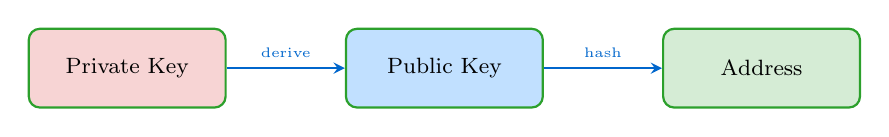
\begin{tikzpicture}[node distance=2cm]
\node[walletbox, fill=dfred!20] (priv) {\footnotesize Private Key};
\node[walletbox, right=1.5cm of priv, fill=dflightblue3] (pub) {\footnotesize Public Key};
\node[walletbox, right=1.5cm of pub, fill=dfgreen!20] (addr) {\footnotesize Address};
\draw[arrow] (priv) -- node[above, font=\tiny] {derive} (pub);
\draw[arrow] (pub) -- node[above, font=\tiny] {hash} (addr);
\end{tikzpicture}
\end{center}

\bottomnote{Key insight: Private key $\rightarrow$ Public key is one-way (cannot reverse)}
\end{frame}

% =======================================================================
% SLIDE 4: PREREQUISITES - DIGITAL SIGNATURES
% =======================================================================
\begin{frame}{Prerequisites: Digital Signatures}
\textbf{How Transactions Get Authorized}

\vspace{3mm}
A \textbf{digital signature} proves that:
\begin{enumerate}\compactlist
\item The owner of the private key authorized this exact transaction
\item The transaction hasn't been modified since signing
\item The signer cannot deny having signed it (non-repudiation)
\end{enumerate}

\vspace{3mm}
\begin{center}
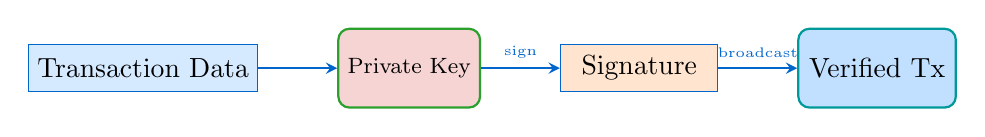
\begin{tikzpicture}[node distance=1.2cm]
\node[txfield, minimum width=2cm] (tx) {Transaction Data};
\node[walletbox, fill=dfred!20, right=1cm of tx, minimum width=1.8cm] (key) {\footnotesize Private Key};
\node[txfield, right=1cm of key, fill=dforange!20, minimum width=2cm] (sig) {Signature};
\node[blocknode, right=1cm of sig, minimum width=2cm] (verify) {Verified Tx};

\draw[arrow] (tx) -- (key);
\draw[arrow] (key) -- node[above, font=\tiny] {sign} (sig);
\draw[arrow] (sig) -- node[above, font=\tiny] {broadcast} (verify);
\end{tikzpicture}
\end{center}

\vspace{3mm}
\textbf{Anyone can verify} a signature using the public key, but \textbf{only the key holder} can create valid signatures.

\begin{block}{Connection to Wallets}
A wallet's primary job is to securely store private keys and use them to sign transactions.
\end{block}
\end{frame}

% =======================================================================
% SLIDE 5: FROM THEORY TO PRACTICE
% =======================================================================
\begin{frame}{From Theory to Practice: How Users Interact}
\begin{center}
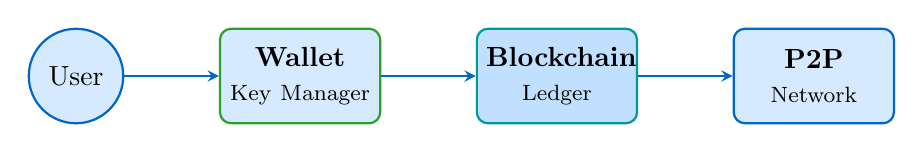
\begin{tikzpicture}[node distance=1cm]
% User
\node[usernode] (user) {User};

% Wallet
\node[walletbox, right=1.2cm of user, minimum width=2cm, minimum height=1.2cm, text width=1.8cm, align=center] (wallet) {
\textbf{Wallet}\\
\footnotesize Key Manager
};

% Blockchain
\node[blocknode, right=1.2cm of wallet, minimum width=2cm, minimum height=1.2cm, text width=1.8cm, align=center] (bc) {
\textbf{Blockchain}\\
\footnotesize Ledger
};

% Network
\node[walletbox, right=1.2cm of bc, minimum width=2cm, minimum height=1.2cm, text width=1.8cm, align=center, draw=dfblue] (network) {
\textbf{P2P}\\
\footnotesize Network
};

\draw[arrow] (user) -- (wallet);
\draw[arrow] (wallet) -- (bc);
\draw[arrow] (bc) -- (network);
\end{tikzpicture}
\end{center}

\vspace{5mm}
\textbf{Key insight:} Users never interact with the blockchain directly.

The \textbf{wallet} is the interface -- it manages keys, signs transactions, and broadcasts them to the network.

\begin{block}{Common Misconception}
Wallets don't ``store'' cryptocurrency. The blockchain stores balances.\\
Wallets store \textit{keys} that prove you can spend those balances.
\end{block}
\end{frame}

% =======================================================================
% SLIDE 6: WHAT IS A WALLET
% =======================================================================
\begin{frame}{What Is a Wallet, Really?}
\begin{columns}[T]
\begin{column}{0.55\textwidth}
\textbf{A wallet is a key management tool}

It does three things:
\begin{enumerate}
\item \textbf{Stores private keys} (securely, hopefully)
\item \textbf{Signs transactions} using those keys
\item \textbf{Broadcasts transactions} to the network
\end{enumerate}

\vspace{3mm}
\textbf{It does NOT:}
\begin{itemize}
\item Store cryptocurrency
\item Connect you to a bank
\item Know your identity
\item Require permission to create
\end{itemize}
\end{column}
\begin{column}{0.42\textwidth}
\begin{center}
\fbox{\parbox{0.9\textwidth}{
\textbf{Wallet Contents}\\[3mm]
\textcolor{dfred}{Private Key 1}\\
{\tiny 0x7a2b...secret}\\[2mm]
\textcolor{dfgreen}{Address 1: 0x9c4d...}\\[1mm]
\textcolor{dfgreen}{Address 2: 0xf3e8...}\\[2mm]
Balance: 1.5 ETH\\
{\tiny (queried from blockchain)}
}}
\end{center}
\end{column}
\end{columns}
\end{frame}

% =======================================================================
% SLIDE 7: WALLET TYPES SPECTRUM
% =======================================================================
\begin{frame}{Types of Wallets: A Spectrum of Tradeoffs}
\begin{center}
\textbf{Security vs. Convenience Tradeoff}

\vspace{3mm}
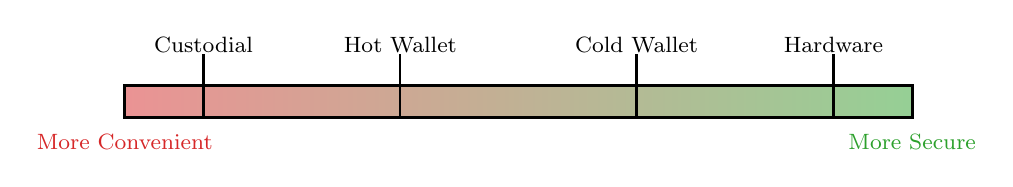
\begin{tikzpicture}
% Spectrum bar
\draw[very thick, left color=dfred!50, right color=dfgreen!50] (-5,-0.2) rectangle (5,0.2);
\node[below=0.3cm, font=\footnotesize] at (-5,0) {\textcolor{dfred}{More Convenient}};
\node[below=0.3cm, font=\footnotesize] at (5,0) {\textcolor{dfgreen}{More Secure}};

% Wallet types
\node[above=0.5cm] at (-4, 0) {\footnotesize Custodial};
\node[above=0.5cm] at (-1.5, 0) {\footnotesize Hot Wallet};
\node[above=0.5cm] at (1.5, 0) {\footnotesize Cold Wallet};
\node[above=0.5cm] at (4, 0) {\footnotesize Hardware};

\draw[thick] (-4, -0.2) -- (-4, 0.6);
\draw[thick] (-1.5, -0.2) -- (-1.5, 0.6);
\draw[thick] (1.5, -0.2) -- (1.5, 0.6);
\draw[thick] (4, -0.2) -- (4, 0.6);
\end{tikzpicture}
\end{center}

\vspace{5mm}
\begin{tabular}{l|l|l|l}
\toprule
\textbf{Type} & \textbf{Key Control} & \textbf{Example} & \textbf{Risk} \\
\midrule
Custodial & Exchange holds keys & Coinbase, Binance & Exchange hack \\
Hot Wallet & You hold, online & MetaMask & Malware, phishing \\
Cold Wallet & You hold, offline & Paper wallet & Physical loss \\
Hardware & You hold, secure chip & Ledger, Trezor & Device failure \\
\bottomrule
\end{tabular}
\end{frame}

% =======================================================================
% SLIDE 8: CUSTODIAL WALLETS EXPLAINED
% =======================================================================
\begin{frame}{Custodial Wallets: Someone Else Holds Your Keys}
\textbf{Definition:} A \textbf{custodial wallet} is one where a third party (typically an exchange) controls the private keys on your behalf.

\vspace{3mm}
\begin{columns}[T]
\begin{column}{0.48\textwidth}
\textbf{How It Works}
\begin{enumerate}\compactlist
\item You create an account with an exchange
\item Exchange generates keys for you
\item You see a balance in your account
\item When you ``send,'' exchange signs
\item You never see the private key
\end{enumerate}

\vspace{3mm}
\textbf{Examples:}
\begin{itemize}\compactlist
\item Coinbase
\item Binance
\item Kraken
\item Crypto.com
\end{itemize}
\end{column}
\begin{column}{0.48\textwidth}
\textbf{Pros and Cons}

\textcolor{dfgreen}{Advantages:}
\begin{itemize}\compactlist
\item Easy to use (like a bank app)
\item Password recovery possible
\item Customer support available
\item Fiat on/off ramps
\end{itemize}

\vspace{2mm}
\textcolor{dfred}{Disadvantages:}
\begin{itemize}\compactlist
\item You don't control your keys
\item Exchange can freeze your funds
\item Exchange can be hacked
\item May require KYC/identity
\end{itemize}
\end{column}
\end{columns}
\end{frame}

% =======================================================================
% SLIDE 9: NON-CUSTODIAL WALLETS
% =======================================================================
\begin{frame}{Non-Custodial Wallets: You Control Your Keys}
\textbf{Definition:} A \textbf{non-custodial wallet} (or self-custody wallet) is one where only you control the private keys.

\vspace{3mm}
\begin{columns}[T]
\begin{column}{0.48\textwidth}
\textbf{How It Works}
\begin{enumerate}\compactlist
\item You generate keys yourself
\item Keys stored on your device
\item You sign all transactions
\item No account required
\item No permission needed
\end{enumerate}

\vspace{3mm}
\textbf{Examples:}
\begin{itemize}\compactlist
\item MetaMask (browser extension)
\item Trust Wallet (mobile)
\item Electrum (Bitcoin)
\item Ledger/Trezor (hardware)
\end{itemize}
\end{column}
\begin{column}{0.48\textwidth}
\textbf{Pros and Cons}

\textcolor{dfgreen}{Advantages:}
\begin{itemize}\compactlist
\item Full control of your funds
\item No counterparty risk
\item Censorship resistant
\item Privacy (no KYC)
\end{itemize}

\vspace{2mm}
\textcolor{dfred}{Disadvantages:}
\begin{itemize}\compactlist
\item You are fully responsible
\item Lose keys = lose funds
\item No customer support
\item Steeper learning curve
\end{itemize}
\end{column}
\end{columns}

\vspace{3mm}
\begin{center}
\fbox{\parbox{0.6\textwidth}{\centering
\textbf{``Not your keys, not your coins''}\\
\footnotesize A fundamental principle of cryptocurrency ownership
}}
\end{center}
\end{frame}

% =======================================================================
% SLIDE 10: HOT VS COLD WALLETS
% =======================================================================
\begin{frame}{Hot vs. Cold Wallets: Internet Connectivity}
\textbf{Key Question:} Is your wallet connected to the internet?

\vspace{5mm}
\begin{columns}[T]
\begin{column}{0.48\textwidth}
\begin{center}
\textbf{Hot Wallet}\\
\textcolor{dforange}{(Internet-connected)}
\end{center}

\begin{itemize}\compactlist
\item Keys stored on online device
\item Computer, phone, browser
\item Ready for immediate use
\item Good for daily transactions
\item \textcolor{dfred}{Vulnerable to hackers}
\end{itemize}

\vspace{2mm}
\textbf{Analogy:} Cash in your pocket -- convenient for daily spending
\end{column}
\begin{column}{0.48\textwidth}
\begin{center}
\textbf{Cold Wallet}\\
\textcolor{dfblue}{(Offline)}
\end{center}

\begin{itemize}\compactlist
\item Keys never touch internet
\item Paper, hardware device, air-gapped computer
\item Requires extra steps to use
\item Good for long-term storage
\item \textcolor{dfgreen}{Much more secure}
\end{itemize}

\vspace{2mm}
\textbf{Analogy:} Money in a safe deposit box -- secure for savings
\end{column}
\end{columns}

\vspace{5mm}
\begin{block}{Best Practice}
Use both: hot wallet for daily use (small amounts), cold storage for savings (large amounts).
\end{block}
\end{frame}

% =======================================================================
% SLIDE 11: HARDWARE WALLETS
% =======================================================================
\begin{frame}{Hardware Wallets: The Gold Standard for Security}
\textbf{Definition:} A \textbf{hardware wallet} is a dedicated physical device that stores private keys offline and signs transactions securely.

\vspace{3mm}
\begin{columns}[T]
\begin{column}{0.55\textwidth}
\textbf{How It Works}
\begin{enumerate}\compactlist
\item Keys generated and stored on device
\item Keys \textit{never} leave the device
\item Transaction data sent to device
\item Device signs internally
\item Only signature returned to computer
\end{enumerate}

\vspace{3mm}
\textbf{Popular Hardware Wallets:}
\begin{itemize}\compactlist
\item Ledger Nano (S/X)
\item Trezor (One/Model T)
\item GridPlus Lattice1
\item Keystone Pro
\end{itemize}
\end{column}
\begin{column}{0.42\textwidth}
\textbf{Security Features}
\begin{itemize}\compactlist
\item Secure element chip
\item PIN code protection
\item Physical confirmation button
\item Display shows transaction details
\item Recovery phrase backup
\end{itemize}

\vspace{3mm}
\textbf{Typical Cost:} \$50--\$200

\vspace{3mm}
\textcolor{dfgreen}{Recommended for:}\\
Anyone holding >\$1,000 in crypto
\end{column}
\end{columns}
\end{frame}

% =======================================================================
% SLIDE 12: SEED PHRASES
% =======================================================================
\begin{frame}{Seed Phrases: Your Master Backup}
\textbf{Definition:} A \textbf{seed phrase} (or recovery phrase) is a list of 12-24 words that can regenerate all your private keys.

\vspace{3mm}
\begin{center}
\fbox{\parbox{0.85\textwidth}{
\texttt{abandon ability able about above absent absorb abstract absurd abuse access accident}
\\[2mm]
\footnotesize This 12-word phrase encodes your entire wallet. Anyone with these words controls your funds.
}}
\end{center}

\vspace{3mm}
\begin{columns}[T]
\begin{column}{0.48\textwidth}
\textbf{How It Works (BIP-39)}
\begin{itemize}\compactlist
\item 2,048 possible words
\item 12 words = 128 bits entropy
\item 24 words = 256 bits entropy
\item Mathematically generates keys
\item One phrase $\rightarrow$ unlimited addresses
\end{itemize}
\end{column}
\begin{column}{0.48\textwidth}
\textbf{Critical Security Rules}
\begin{itemize}\compactlist
\item \textcolor{dfred}{NEVER share with anyone}
\item \textcolor{dfred}{NEVER type into a website}
\item \textcolor{dfred}{NEVER store digitally}
\item Write on paper or metal
\item Store in multiple secure locations
\end{itemize}
\end{column}
\end{columns}

\bottomnote{Lose your seed phrase + lose your device = permanently lose all funds}
\end{frame}

% =======================================================================
% SLIDE 13: CUSTODIAL VS NON-CUSTODIAL COMPARISON
% =======================================================================
\begin{frame}{Custodial vs. Non-Custodial: Direct Comparison}
\begin{columns}[T]
\begin{column}{0.48\textwidth}
\textbf{Custodial (Exchange) Wallet}

You $\rightarrow$ Exchange $\rightarrow$ Blockchain

\vspace{3mm}
\begin{itemize}\compactlist
\item \textcolor{dfgreen}{Easy to use}
\item \textcolor{dfgreen}{Password recovery possible}
\item \textcolor{dfgreen}{Fiat on/off ramps}
\item \textcolor{dfred}{You don't control keys}
\item \textcolor{dfred}{Exchange can freeze funds}
\item \textcolor{dfred}{Exchange can be hacked}
\end{itemize}
\end{column}
\begin{column}{0.48\textwidth}
\textbf{Non-Custodial (Self-Custody)}

You $\rightarrow$ Your Wallet $\rightarrow$ Blockchain

\vspace{3mm}
\begin{itemize}\compactlist
\item \textcolor{dfgreen}{Full control}
\item \textcolor{dfgreen}{No counterparty risk}
\item \textcolor{dfgreen}{Censorship resistant}
\item \textcolor{dfred}{You are responsible}
\item \textcolor{dfred}{Lose keys = lose funds}
\item \textcolor{dfred}{No customer support}
\end{itemize}
\end{column}
\end{columns}

\vspace{5mm}
\begin{center}
\fbox{\parbox{0.6\textwidth}{\centering
\textbf{FTX Collapse (2022)}\\
\footnotesize \$8 billion in customer funds lost when exchange failed.\\
Customers using custodial wallets had no recourse.
}}
\end{center}
\end{frame}

% =======================================================================
% SLIDE 14: TRANSACTION DEFINITION
% =======================================================================
\begin{frame}{What Is a Blockchain Transaction?}
\textbf{Definition:} A \textbf{transaction} is a signed message that transfers value or triggers computation on a blockchain.

\vspace{5mm}
\begin{center}
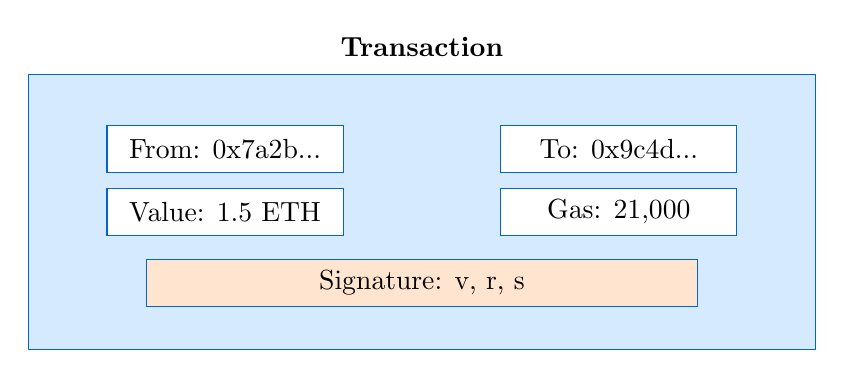
\begin{tikzpicture}[node distance=0.8cm]
% Transaction box
\node[txfield, minimum width=10cm, minimum height=3.5cm, fill=dflightblue4] (txbox) {};
\node[above=0.1cm of txbox.north, font=\bfseries] {Transaction};

% Fields inside
\node[txfield, minimum width=3cm, fill=white] at (-2.5, 0.8) (from) {From: 0x7a2b...};
\node[txfield, minimum width=3cm, fill=white] at (2.5, 0.8) (to) {To: 0x9c4d...};
\node[txfield, minimum width=3cm, fill=white] at (-2.5, 0) (value) {Value: 1.5 ETH};
\node[txfield, minimum width=3cm, fill=white] at (2.5, 0) (gas) {Gas: 21,000};
\node[txfield, minimum width=7cm, fill=dforange!20] at (0, -0.9) (sig) {Signature: v, r, s};
\end{tikzpicture}
\end{center}

\vspace{3mm}
\textbf{Key Components:}
\begin{itemize}\compactlist
\item \textbf{From:} Sender's address (derived from signature)
\item \textbf{To:} Recipient's address
\item \textbf{Value:} Amount to transfer
\item \textbf{Gas:} Computational budget
\item \textbf{Signature:} Cryptographic proof of authorization
\end{itemize}
\end{frame}

% =======================================================================
% SLIDE 15: ANATOMY OF A TRANSACTION
% =======================================================================
\begin{frame}{Anatomy of a Blockchain Transaction}
\begin{center}
\textbf{Ethereum Transaction Structure}

\vspace{3mm}
\begin{tabular}{|l|l|l|}
\hline
\textbf{Field} & \textbf{Example Value} & \textbf{Purpose} \\
\hline
From & 0x7a2b...9f3c & Sender's address \\
To & 0x9c4d...e8f2 & Recipient's address \\
Value & 1.5 ETH & Amount to transfer \\
Nonce & 42 & Transaction count (prevents replay) \\
Gas Limit & 21,000 & Maximum computation units \\
Gas Price & 50 gwei & Price per gas unit (see frame 18) \\
\hline
\textbf{Signature} & v, r, s & Proves authorization \\
\hline
\end{tabular}
\end{center}

\vspace{5mm}
The signature covers ALL fields above it -- proving the sender authorized \textit{this exact transaction}.

\begin{block}{What is a Nonce?}
The nonce is a counter that tracks how many transactions you've sent. It prevents attackers from replaying old transactions and ensures transactions are processed in order.
\end{block}
\end{frame}

% =======================================================================
% SLIDE 16: TRANSACTION LIFECYCLE
% =======================================================================
\begin{frame}{Transaction Lifecycle: From Creation to Confirmation}
\begin{center}
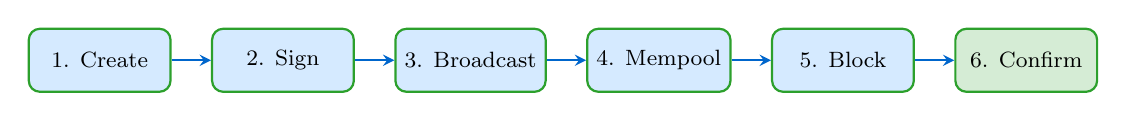
\begin{tikzpicture}[node distance=0.8cm, font=\footnotesize]
% Steps
\node[walletbox, minimum width=1.8cm, minimum height=0.8cm] (create) {1. Create};
\node[walletbox, minimum width=1.8cm, minimum height=0.8cm, right=0.5cm of create] (sign) {2. Sign};
\node[walletbox, minimum width=1.8cm, minimum height=0.8cm, right=0.5cm of sign] (broadcast) {3. Broadcast};
\node[walletbox, minimum width=1.8cm, minimum height=0.8cm, right=0.5cm of broadcast] (mempool) {4. Mempool};
\node[walletbox, minimum width=1.8cm, minimum height=0.8cm, right=0.5cm of mempool] (block) {5. Block};
\node[walletbox, minimum width=1.8cm, minimum height=0.8cm, fill=dfgreen!20, right=0.5cm of block] (confirm) {6. Confirm};

\draw[arrow] (create) -- (sign);
\draw[arrow] (sign) -- (broadcast);
\draw[arrow] (broadcast) -- (mempool);
\draw[arrow] (mempool) -- (block);
\draw[arrow] (block) -- (confirm);
\end{tikzpicture}
\end{center}

\vspace{3mm}
\begin{enumerate}\compactlist
\item \textbf{Create:} Wallet builds transaction with recipient, amount, gas
\item \textbf{Sign:} Private key creates digital signature
\item \textbf{Broadcast:} Transaction sent to network nodes
\item \textbf{Mempool:} Waits in ``waiting room'' for inclusion
\item \textbf{Block:} Miner/validator includes in a block
\item \textbf{Confirm:} Block added to chain; more blocks = more confirmations
\end{enumerate}

\vspace{3mm}
\begin{block}{Mempool Definition}
The \textbf{mempool} (memory pool) is where valid but unconfirmed transactions wait before being included in a block. Each node maintains its own mempool.
\end{block}
\end{frame}

% =======================================================================
% SLIDE 17: UNDERSTANDING GAS
% =======================================================================
\begin{frame}{Understanding Gas: The Cost of Computation}
\begin{columns}[T]
\begin{column}{0.55\textwidth}
\textbf{What is Gas?}
\begin{itemize}\compactlist
\item Unit measuring computational work
\item Each operation has a gas cost
\item Simple transfer: 21,000 gas
\item Smart contract call: varies (100K+)
\end{itemize}

\vspace{3mm}
\textbf{Gas Economics}

\textbf{Analogy:} Gas limit = max fuel in tank; Gas price = cost per gallon

\[
\text{Fee} = \text{Gas Used} \times \text{Gas Price}
\]

\vspace{2mm}
\textbf{Example:}
\begin{itemize}\compactlist
\item Gas used: 21,000
\item Gas price: 50 gwei (explained in detail on next frame)
\item Fee = 21,000 $\times$ 50 gwei = 0.00105 ETH
\end{itemize}
\end{column}
\begin{column}{0.42\textwidth}
\textbf{Why Gas Exists}
\begin{enumerate}\compactlist
\item Prevents infinite loops
\item Compensates validators
\item Prioritizes transactions
\item Allocates scarce block space
\end{enumerate}

\vspace{3mm}
\begin{center}
\fbox{\parbox{0.9\textwidth}{
\textbf{Network Congestion}\\[2mm]
High demand $\rightarrow$\\
Higher gas prices $\rightarrow$\\
Higher fees\\[2mm]
\footnotesize (Supply and demand)
}}
\end{center}
\end{column}
\end{columns}

\bottomnote{Gas prices fluctuate wildly -- from cents to hundreds of dollars per transaction}
\end{frame}

% =======================================================================
% SLIDE 18: GAS PRICE UNITS
% =======================================================================
\begin{frame}{Gas Price Units: Gwei Explained}
\textbf{Definition:} \textbf{Gwei} (giga-wei) is the standard unit for measuring gas prices on Ethereum.

\vspace{3mm}
\textbf{Think of it like cents to dollars, but with more decimal places:}\\
Wei is the smallest unit (like a penny's fraction), and ETH is the whole unit (like a dollar).

\vspace{3mm}
\begin{center}
\begin{tabular}{l|l|l}
\toprule
\textbf{Unit} & \textbf{Value in Wei} & \textbf{Value in ETH} \\
\midrule
Wei & 1 & 0.000000000000000001 ETH \\
Gwei & 1,000,000,000 & 0.000000001 ETH \\
ETH & 1,000,000,000,000,000,000 & 1 ETH \\
\bottomrule
\end{tabular}
\end{center}

\vspace{5mm}
\textbf{Typical Gas Prices:}
\begin{itemize}\compactlist
\item \textbf{Low activity:} 10-20 gwei
\item \textbf{Normal activity:} 30-50 gwei
\item \textbf{High congestion:} 100-200+ gwei
\item \textbf{NFT drop/DeFi rush:} 500+ gwei
\end{itemize}

\vspace{3mm}
\begin{block}{Quick Calculation}
At 50 gwei, a simple ETH transfer costs: $21,000 \times 50 = 1,050,000$ gwei = 0.00105 ETH\\
If ETH = \$2,000, that's about \$2.10 per transaction.
\end{block}
\end{frame}

% =======================================================================
% SLIDE 19: EIP-1559 FEE STRUCTURE
% =======================================================================
\begin{frame}{EIP-1559: Modern Ethereum Fee Structure}
\textbf{EIP-1559} was a major 2021 upgrade that changed how Ethereum calculates transaction fees.

\vspace{2mm}
\textbf{Since August 2021}, Ethereum uses a two-part fee system:

\vspace{3mm}
\begin{columns}[T]
\begin{column}{0.48\textwidth}
\textbf{Base Fee}
\begin{itemize}\compactlist
\item Algorithmically determined
\item Adjusts based on congestion
\item \textcolor{dfred}{Burned} (not paid to validators)
\item Creates deflationary pressure
\end{itemize}
\end{column}
\begin{column}{0.48\textwidth}
\textbf{Priority Fee (Tip)}
\begin{itemize}\compactlist
\item Optional tip to validator
\item Incentivizes faster inclusion
\item \textcolor{dfgreen}{Paid to validator}
\item Higher tip = faster confirmation
\end{itemize}
\end{column}
\end{columns}

\vspace{5mm}
\begin{center}
\fbox{\parbox{0.7\textwidth}{\centering
\textbf{Total Fee Formula}\\[2mm]
$\text{Fee} = (\text{Base Fee} + \text{Priority Fee}) \times \text{Gas Used}$\\[2mm]
\footnotesize Example: $(20 + 2) \times 21,000 = 462,000$ gwei = 0.000462 ETH
}}
\end{center}

\vspace{3mm}
\textbf{Benefit:} More predictable fees. Base fee adjusts smoothly instead of wild bidding wars.
\end{frame}

% =======================================================================
% SLIDE 20: TRANSACTION CONFIRMATIONS
% =======================================================================
\begin{frame}{Transaction Confirmations: When Is It Final?}
\textbf{Definition:} A \textbf{confirmation} occurs each time a new block is added after the block containing your transaction.

\vspace{3mm}
\begin{center}
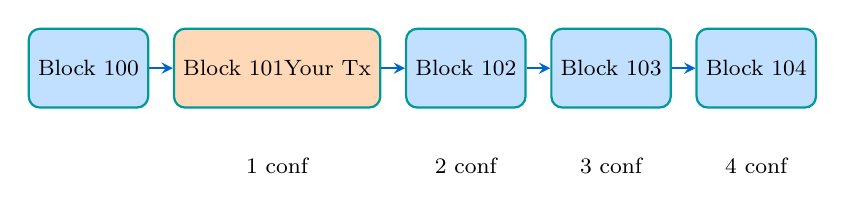
\begin{tikzpicture}[node distance=0.3cm, font=\footnotesize]
\node[blocknode, minimum width=1.5cm] (b1) {Block 100};
\node[blocknode, minimum width=1.5cm, right=0.3cm of b1, fill=dforange!30] (b2) {Block 101\\Your Tx};
\node[blocknode, minimum width=1.5cm, right=0.3cm of b2] (b3) {Block 102};
\node[blocknode, minimum width=1.5cm, right=0.3cm of b3] (b4) {Block 103};
\node[blocknode, minimum width=1.5cm, right=0.3cm of b4] (b5) {Block 104};

\draw[arrow] (b1) -- (b2);
\draw[arrow] (b2) -- (b3);
\draw[arrow] (b3) -- (b4);
\draw[arrow] (b4) -- (b5);

\node[below=0.5cm of b2] {1 conf};
\node[below=0.5cm of b3] {2 conf};
\node[below=0.5cm of b4] {3 conf};
\node[below=0.5cm of b5] {4 conf};
\end{tikzpicture}
\end{center}

\vspace{3mm}
\begin{tabular}{l|l|l}
\toprule
\textbf{Blockchain} & \textbf{Recommended} & \textbf{Time} \\
\midrule
Bitcoin & 6 confirmations & $\sim$60 minutes \\
Ethereum (PoS) & 2 epochs (finality) & $\sim$15 minutes \\
Ethereum (small amounts) & 12 confirmations & $\sim$3 minutes \\
\bottomrule
\end{tabular}

\vspace{3mm}
\textbf{Why wait?} More confirmations = harder to reverse. Protects against chain reorganizations.
\end{frame}

% =======================================================================
% SLIDE 21: UTXO VS ACCOUNT MODEL
% =======================================================================
\begin{frame}{Two Models: UTXO vs. Account-Based}
\textbf{How does the blockchain track who owns what?}

\vspace{3mm}
\begin{columns}[T]
\begin{column}{0.48\textwidth}
\textbf{UTXO Model (Bitcoin)}

Unspent Transaction Outputs

\begin{itemize}\compactlist
\item Balance = sum of unspent outputs
\item Must spend entire UTXO
\item Creates ``change'' outputs
\item Better for privacy
\item Better for parallelization
\end{itemize}

\vspace{2mm}
\textbf{Analogy:} Cash bills\\
You can't tear a \$10 bill
\end{column}
\begin{column}{0.48\textwidth}
\textbf{Account Model (Ethereum)}

Like a bank account

\begin{itemize}\compactlist
\item Balance stored directly
\item Can send any amount
\item No change needed
\item Simpler to understand
\item Better for smart contracts
\end{itemize}

\vspace{2mm}
\textbf{Analogy:} Bank account\\
Balance adjusted up/down
\end{column}
\end{columns}

\vspace{5mm}
\begin{block}{UTXO Example}
Alice has 0.5 BTC (one UTXO). To send 0.3 BTC: she spends the entire 0.5 BTC UTXO, sends 0.3 BTC to Bob, and 0.2 BTC back to herself as ``change.''
\end{block}
\end{frame}

% =======================================================================
% SLIDE 22: THE UX GAP
% =======================================================================
\begin{frame}{The User Experience Gap}
\begin{center}
\textbf{What crypto asks users to understand:}
\end{center}

\begin{columns}[T]
\begin{column}{0.48\textwidth}
\begin{center}
\textbf{Traditional Banking}
\end{center}
\begin{itemize}\compactlist
\item Username and password
\item ``Forgot password?'' link
\item Customer support
\item FDIC insurance
\item Fraud protection
\item Clear error messages
\end{itemize}

\vspace{3mm}
\begin{center}
\textcolor{dfgreen}{Forgiving of mistakes}
\end{center}
\end{column}
\begin{column}{0.48\textwidth}
\begin{center}
\textbf{Cryptocurrency}
\end{center}
\begin{itemize}\compactlist
\item 24-word seed phrase
\item Lose phrase = lose everything
\item No customer support
\item No insurance (usually)
\item Irreversible transactions
\item Cryptic error: ``insufficient gas''
\end{itemize}

\vspace{3mm}
\begin{center}
\textcolor{dfred}{Unforgiving of mistakes}
\end{center}
\end{column}
\end{columns}

\vspace{3mm}
\begin{block}{The UX Problem}
Crypto's security model requires users to be their own bank.\\
Most people don't want that responsibility.
\end{block}
\end{frame}

% =======================================================================
% SLIDE 23: COMMON USER ERRORS
% =======================================================================
\begin{frame}{Common User Errors (And Their Consequences)}
\begin{center}
\begin{tabular}{l|l|l}
\toprule
\textbf{Error} & \textbf{Consequence} & \textbf{Recovery?} \\
\midrule
Lost seed phrase & Permanent loss of funds & \textcolor{dfred}{No} \\
Sent to wrong address & Funds gone forever & \textcolor{dfred}{No} \\
Wrong network (ETH to BSC) & Funds stuck/lost & \textcolor{dforange}{Sometimes} \\
Insufficient gas & Transaction fails & \textcolor{dfgreen}{Yes, retry} \\
Approved malicious contract & Wallet drained & \textcolor{dfred}{No} \\
Phishing attack & Keys stolen & \textcolor{dfred}{No} \\
Didn't verify contract & Funds stolen & \textcolor{dfred}{No} \\
\bottomrule
\end{tabular}
\end{center}

\vspace{5mm}
\textbf{Scale of the problem:}
\begin{itemize}
\item \$3.8 billion lost to crypto hacks in 2022 (Chainalysis)
\item Estimated 20\% of Bitcoin permanently inaccessible (lost keys)
\item Phishing remains the \#1 attack vector
\end{itemize}
\end{frame}

% =======================================================================
% SLIDE 24: IMPROVING CRYPTO UX
% =======================================================================
\begin{frame}{Improving Crypto UX: Current Efforts}
\begin{columns}[T]
\begin{column}{0.48\textwidth}
\textbf{Technical Solutions}
\begin{itemize}\compactlist
\item \textbf{Account abstraction:} Smart contract wallets with recovery
\item \textbf{Social recovery:} Trusted friends can help recover
\item \textbf{Multi-sig:} Require multiple keys to transact
\item \textbf{Hardware wallets:} Secure key storage
\item \textbf{ENS names:} Human-readable addresses (e.g., alice.eth)
\end{itemize}
\end{column}
\begin{column}{0.48\textwidth}
\textbf{UX Improvements}
\begin{itemize}\compactlist
\item \textbf{Transaction simulation:} Show what will happen before signing
\item \textbf{Clear warnings:} ``This will drain your wallet''
\item \textbf{Gas estimation:} Show fees in dollars
\item \textbf{Address books:} Saved, verified addresses
\item \textbf{Better error messages:} Human-readable explanations
\end{itemize}
\end{column}
\end{columns}

\vspace{5mm}
\begin{block}{The Goal}
Make self-custody as easy as using a bank app, without sacrificing security or decentralization.
\end{block}
\end{frame}

% =======================================================================
% SLIDE 25: HANDS-ON EXERCISE INTRO
% =======================================================================
\begin{frame}{Hands-On Exercise: Blockchain Transaction Analysis}
\begin{center}
\textbf{NB07: Blockchain Transactions}
\end{center}

\vspace{3mm}
In the accompanying Jupyter notebook, you will:

\begin{enumerate}
\item \textbf{Build a transaction} from scratch with all required fields
\item \textbf{Calculate gas fees} for different types of operations
\item \textbf{Compare UTXO vs. Account models} through examples
\item \textbf{Analyze transaction lifecycle} from creation to confirmation
\item \textbf{Simulate fee markets} under different network conditions
\end{enumerate}

\vspace{5mm}
\begin{block}{Learning Goals}
\begin{itemize}
\item Understand transaction structure at a technical level
\item Practice fee calculations (gas units $\times$ gas price)
\item See how the mempool works
\item Compare Bitcoin and Ethereum transaction models
\end{itemize}
\end{block}
\end{frame}

% =======================================================================
% SLIDE 26: HANDS-ON EXERCISE PREVIEW
% =======================================================================
\begin{frame}[fragile]{Hands-On: Code Preview}
\textbf{Example from NB07: Building a Transaction}

\vspace{3mm}
\begin{lstlisting}[style=pythonstyle]
# Transaction structure (simplified)
transaction = {
    "from": "0x742d35Cc6634C0532925a3b844Bc9e7595f8aB12",
    "to": "0x8Ba1f109551bD432803012645Ac136ddd64DBA72",
    "value": 1.5,  # ETH
    "gas_limit": 21000,  # Standard transfer
    "gas_price": 50,  # Gwei
    "nonce": 42
}

# Calculate transaction fee
fee_gwei = transaction["gas_limit"] * transaction["gas_price"]
fee_eth = fee_gwei / 1e9
print(f"Transaction fee: {fee_eth} ETH")
\end{lstlisting}

\vspace{3mm}
\textbf{Output:} Transaction fee: 0.00105 ETH

\vspace{3mm}
\textbf{Try it:} Open NB07 and experiment with different gas prices!
\end{frame}

% =======================================================================
% SLIDE 27: DISCUSSION - WALLET CHOICE
% =======================================================================
\begin{frame}{Discussion: Choosing the Right Wallet}
\textbf{Scenario Analysis}

\vspace{3mm}
\textbf{Consider these users -- which wallet type would you recommend?}

\vspace{3mm}
\begin{enumerate}
\item \textbf{Alice} is new to crypto and wants to buy \$100 of Bitcoin to hold for years.

\item \textbf{Bob} is a DeFi power user who interacts with smart contracts daily.

\item \textbf{Carol} runs a crypto hedge fund and manages \$10 million in assets.

\item \textbf{Dave} lives in a country with capital controls and needs censorship resistance.
\end{enumerate}

\vspace{5mm}
\begin{block}{Discussion Questions}
\begin{itemize}
\item What factors should each person prioritize?
\item How does the amount at stake affect the choice?
\item When does convenience outweigh security (and vice versa)?
\end{itemize}
\end{block}
\end{frame}

% =======================================================================
% SLIDE 28: DISCUSSION - FEE STRATEGIES
% =======================================================================
\begin{frame}{Discussion: Transaction Fee Strategies}
\textbf{When to pay more, when to pay less}

\vspace{3mm}
\begin{columns}[T]
\begin{column}{0.48\textwidth}
\textbf{Scenario 1: Urgent Transfer}
\begin{itemize}\compactlist
\item You need to deposit ETH to an exchange to sell before price drops
\item Network is congested
\item Current gas: 100 gwei
\item What gas price do you set?
\end{itemize}
\end{column}
\begin{column}{0.48\textwidth}
\textbf{Scenario 2: Non-Urgent Transfer}
\begin{itemize}\compactlist
\item You're moving crypto to cold storage
\item No time pressure
\item Current gas: 50 gwei
\item What gas price do you set?
\end{itemize}
\end{column}
\end{columns}

\vspace{5mm}
\textbf{Advanced Strategies:}
\begin{itemize}\compactlist
\item \textbf{Wait for low traffic:} Weekends, late night (UTC)
\item \textbf{Use gas trackers:} etherscan.io/gastracker
\item \textbf{Transaction batching:} Combine multiple sends
\item \textbf{Replace-by-Fee (RBF):} Speed up stuck transactions
\end{itemize}
\end{frame}

% =======================================================================
% SLIDE 29: APPLICATION - REAL WORLD
% =======================================================================
\begin{frame}{Real-World Application: Exchange Withdrawal}
\textbf{What actually happens when you withdraw from Coinbase?}

\vspace{3mm}
\begin{enumerate}\compactlist
\item You request withdrawal to your wallet address
\item Exchange verifies your identity/2FA
\item Exchange creates transaction from \textit{their} wallet
\item Exchange signs with \textit{their} private key
\item Transaction enters mempool
\item Included in block (1 confirmation)
\item More blocks added (6 confirmations for Bitcoin)
\item Your wallet shows the balance
\end{enumerate}

\vspace{3mm}
\begin{block}{Key Insight}
During this entire process, \textbf{you never touched the blockchain}.\\
You asked the exchange to make a transaction on your behalf.\\
This is why you don't control custodial funds -- you're asking permission.
\end{block}
\end{frame}

% =======================================================================
% SLIDE 30: APPLICATION - SECURITY CHECKLIST
% =======================================================================
\begin{frame}{Application: Personal Security Checklist}
\textbf{Before using any cryptocurrency wallet:}

\vspace{3mm}
\begin{columns}[T]
\begin{column}{0.48\textwidth}
\textbf{Setup Phase}
\begin{itemize}\compactlist
\item[$\square$] Generated seed phrase offline?
\item[$\square$] Written on paper (not digital)?
\item[$\square$] Stored in secure location?
\item[$\square$] Made backup copy?
\item[$\square$] Tested recovery process?
\end{itemize}

\vspace{3mm}
\textbf{Daily Use}
\begin{itemize}\compactlist
\item[$\square$] Verify addresses before sending
\item[$\square$] Start with small test transaction
\item[$\square$] Check network before confirming
\item[$\square$] Review contract permissions
\end{itemize}
\end{column}
\begin{column}{0.48\textwidth}
\textbf{Red Flags to Avoid}
\begin{itemize}\compactlist
\item[$\times$] Anyone asking for seed phrase
\item[$\times$] ``Support'' DMs on social media
\item[$\times$] Websites asking to ``verify'' wallet
\item[$\times$] Free token airdrops (often scams)
\item[$\times$] Urgent ``limited time'' offers
\end{itemize}

\vspace{3mm}
\textbf{Best Practices}
\begin{itemize}\compactlist
\item[$\checkmark$] Use hardware wallet for large amounts
\item[$\checkmark$] Enable all security features
\item[$\checkmark$] Keep software updated
\item[$\checkmark$] Never share private keys
\end{itemize}
\end{column}
\end{columns}
\end{frame}

% =======================================================================
% SLIDE 31: EXECUTIVE SUMMARY
% =======================================================================
\begin{frame}{Executive Summary}
\textbf{Key Takeaways from Topic 3.3}

\vspace{5mm}
\begin{enumerate}
\item \textbf{Wallets don't store crypto} -- they store private keys that prove you can spend funds recorded on the blockchain.

\item \textbf{Wallet choice is a security/convenience tradeoff} -- custodial wallets are easy but risky; self-custody is secure but demanding.

\item \textbf{``Not your keys, not your coins''} -- if someone else holds your keys (exchanges), they control your funds.

\item \textbf{Transactions require gas} -- fees are calculated as gas units $\times$ gas price, and fluctuate with network demand.

\item \textbf{The UX gap is real} -- crypto demands users be their own bank, but most people aren't ready for that responsibility.
\end{enumerate}

\vspace{5mm}
\begin{center}
\fbox{\parbox{0.8\textwidth}{\centering
\textbf{Bottom Line:} Understanding wallets and transactions is essential for safely participating in the blockchain ecosystem.
}}
\end{center}
\end{frame}

% =======================================================================
% SLIDE 32: CONCEPT MAP
% =======================================================================
\begin{frame}{Concept Map: The Wallet Ecosystem}
\begin{center}
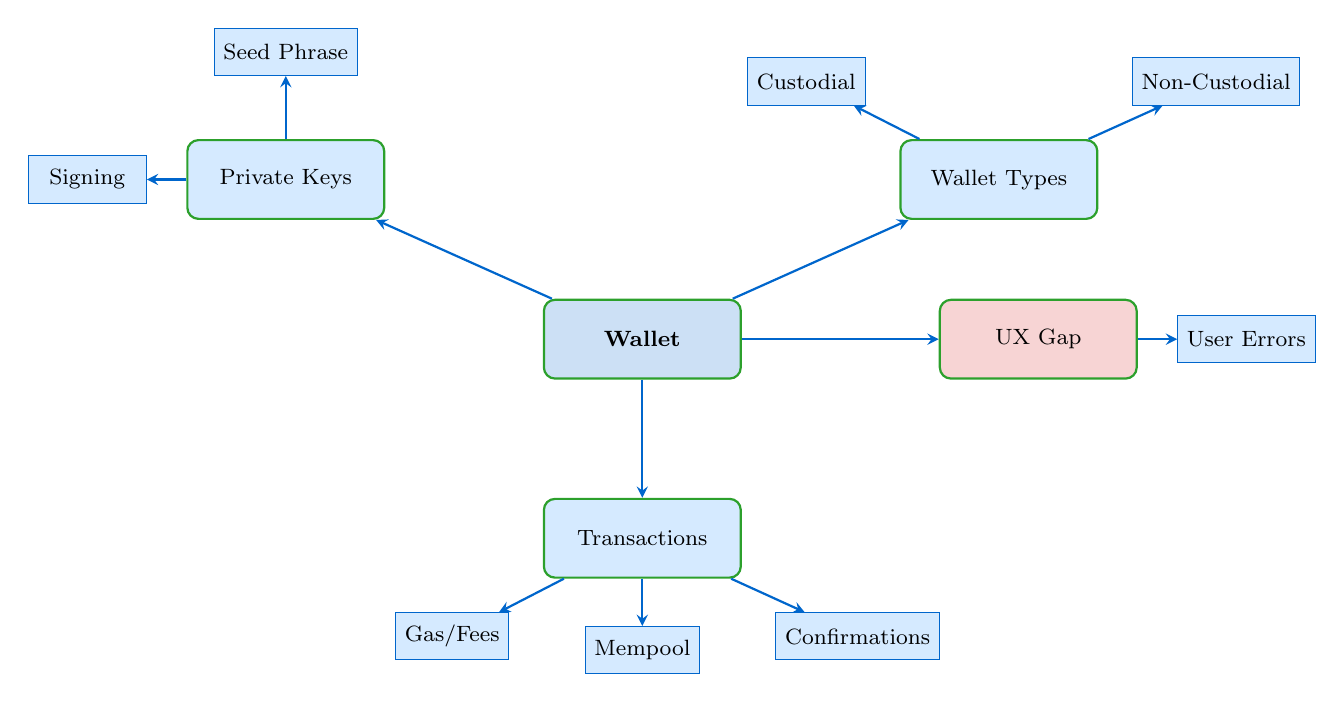
\begin{tikzpicture}[
    node distance=1cm,
    every node/.style={font=\footnotesize},
    level 1/.style={sibling distance=4cm},
    level 2/.style={sibling distance=2cm}
]

% Central node
\node[walletbox, fill=dfblue!20, minimum width=2.5cm] (wallet) {\textbf{Wallet}};

% Key management branch
\node[walletbox, above left=1cm and 2cm of wallet] (keys) {Private Keys};
\node[txfield, above=0.8cm of keys, minimum width=1.8cm] (seed) {Seed Phrase};
\node[txfield, left=0.5cm of keys, minimum width=1.5cm] (sign) {Signing};

% Wallet types branch
\node[walletbox, above right=1cm and 2cm of wallet] (types) {Wallet Types};
\node[txfield, above left=0.6cm of types, minimum width=1.5cm] (cust) {Custodial};
\node[txfield, above right=0.6cm of types, minimum width=1.5cm] (noncust) {Non-Custodial};

% Transaction branch
\node[walletbox, below=1.5cm of wallet] (tx) {Transactions};
\node[txfield, below left=0.6cm of tx, minimum width=1.3cm] (gas) {Gas/Fees};
\node[txfield, below=0.6cm of tx, minimum width=1.3cm] (mempool) {Mempool};
\node[txfield, below right=0.6cm of tx, minimum width=1.3cm] (confirm) {Confirmations};

% UX branch
\node[walletbox, right=2.5cm of wallet, fill=dfred!20] (ux) {UX Gap};
\node[txfield, right=0.5cm of ux, minimum width=1.5cm] (errors) {User Errors};

% Connections
\draw[arrow] (wallet) -- (keys);
\draw[arrow] (wallet) -- (types);
\draw[arrow] (wallet) -- (tx);
\draw[arrow] (wallet) -- (ux);
\draw[arrow] (keys) -- (seed);
\draw[arrow] (keys) -- (sign);
\draw[arrow] (types) -- (cust);
\draw[arrow] (types) -- (noncust);
\draw[arrow] (tx) -- (gas);
\draw[arrow] (tx) -- (mempool);
\draw[arrow] (tx) -- (confirm);
\draw[arrow] (ux) -- (errors);

\end{tikzpicture}
\end{center}
\end{frame}

% =======================================================================
% SLIDE 33: KEY TERMS (1)
% =======================================================================
\begin{frame}{Key Terms \& Definitions (1/2)}
\begin{description}
\item[Wallet] A software or hardware tool that stores private keys and enables signing and broadcasting transactions.

\item[Custodial Wallet] A wallet where a third party (e.g., exchange) controls the private keys on the user's behalf.

\item[Non-Custodial Wallet] A wallet where only the user controls the private keys (self-custody).

\item[Hot Wallet] A wallet connected to the internet, convenient but more vulnerable to attacks.

\item[Cold Wallet] A wallet that stores keys offline, more secure but less convenient for frequent transactions.
\end{description}
\end{frame}

% =======================================================================
% SLIDE 34: KEY TERMS (2)
% =======================================================================
\begin{frame}{Key Terms \& Definitions (2/2)}
\begin{description}
\item[Seed Phrase] A 12-24 word recovery phrase (BIP-39) that can regenerate all private keys in a wallet.

\item[Gas] A unit measuring computational work on Ethereum; each operation costs a specific amount of gas.

\item[Gwei] A denomination of ETH ($10^{-9}$ ETH) commonly used to express gas prices.

\item[Mempool] The ``waiting room'' where valid but unconfirmed transactions wait before being included in a block.

\item[Confirmation] Each new block added after the block containing your transaction; more confirmations = more security.

\item[UTXO] Unspent Transaction Output -- Bitcoin's model for tracking ownership of coins.
\end{description}
\end{frame}

% =======================================================================
% SLIDE 35: COMMON MISCONCEPTIONS
% =======================================================================
\begin{frame}{Common Misconceptions}
\textbf{Myth vs. Reality}

\vspace{5mm}
\begin{enumerate}
\item \textbf{Myth:} ``My wallet stores my cryptocurrency.''\\
\textcolor{dfgreen}{\textbf{Reality:}} Your wallet stores \textit{private keys}. The cryptocurrency exists as records on the blockchain.

\vspace{3mm}
\item \textbf{Myth:} ``If I lose my password, the exchange can help me recover my funds.''\\
\textcolor{dfgreen}{\textbf{Reality:}} True for custodial wallets (exchange holds keys). False for non-custodial wallets -- lose your seed phrase, lose everything.

\vspace{3mm}
\item \textbf{Myth:} ``Blockchain transactions can be reversed if there's fraud.''\\
\textcolor{dfgreen}{\textbf{Reality:}} Blockchain transactions are \textit{irreversible by design}. There's no ``chargeback'' like credit cards.

\vspace{3mm}
\item \textbf{Myth:} ``Hardware wallets are unhackable.''\\
\textcolor{dfgreen}{\textbf{Reality:}} Hardware wallets significantly reduce risk but aren't perfect. Physical theft, supply chain attacks, and user error can still lead to loss.
\end{enumerate}
\end{frame}

% =======================================================================
% SLIDE 36: SELF-ASSESSMENT (1)
% =======================================================================
\begin{frame}{Self-Assessment Questions (1/2)}
\textbf{Question 1:} In Bitcoin's UTXO model, what happens when Alice wants to send 0.3 BTC but only has a single UTXO of 0.5 BTC?

\vspace{3mm}
\begin{enumerate}[A.]
\item The transaction is rejected because the amounts don't match exactly
\item She creates a transaction with the 0.5 BTC UTXO as input, 0.3 BTC to the recipient, and 0.2 BTC back to herself as change
\item The blockchain automatically splits the UTXO into smaller pieces before sending
\item The remaining 0.2 BTC is automatically sent to miners as a fee
\end{enumerate}

\vspace{5mm}
\pause
\textbf{Answer: B}

\textit{In the UTXO model, transaction inputs must consume entire UTXOs. Alice must spend the full 0.5 BTC and explicitly create a ``change'' output returning 0.2 BTC to herself.}
\end{frame}

% =======================================================================
% SLIDE 37: SELF-ASSESSMENT (2)
% =======================================================================
\begin{frame}{Self-Assessment Questions (2/2)}
\textbf{Question 2:} What is the mempool in blockchain networks?

\vspace{2mm}
\begin{enumerate}[A.]
\item A secure storage location for private keys
\item A waiting area where unconfirmed transactions are held before being included in a block
\item A permanent archive of all historical transactions
\item A pool of rewards distributed to miners
\end{enumerate}

\vspace{3mm}
\pause
\textbf{Answer: B} -- \textit{The mempool is where valid but unconfirmed transactions wait.}

\vspace{5mm}
\textbf{Question 3:} What factors determine the size (and thus cost) of a blockchain transaction?

\vspace{2mm}
\begin{enumerate}[A.]
\item The transaction amount and the recipient's location
\item The number of inputs, outputs, and additional data (like smart contract calls)
\item The time of day and network traffic only
\item The cryptocurrency price and market volatility
\end{enumerate}

\vspace{3mm}
\pause
\textbf{Answer: B} -- \textit{Transaction size depends on its data structure, not the amount sent.}
\end{frame}

% =======================================================================
% SLIDE 38: WHAT'S NEXT
% =======================================================================
\begin{frame}{What's Next: Topic 3.4 -- Bitcoin vs. Ethereum}
\textbf{Preview of the next topic:}

\vspace{5mm}
\begin{columns}[T]
\begin{column}{0.48\textwidth}
\textbf{Bitcoin}
\begin{itemize}\compactlist
\item ``Digital Gold'' philosophy
\item Store of value focus
\item UTXO model (as we learned)
\item Limited scripting
\item Conservative development
\end{itemize}
\end{column}
\begin{column}{0.48\textwidth}
\textbf{Ethereum}
\begin{itemize}\compactlist
\item ``World Computer'' vision
\item Smart contract platform
\item Account model
\item Turing-complete programming (see Topic 3.4 for full explanation)
\item Rapid innovation
\end{itemize}
\end{column}
\end{columns}

\vspace{5mm}
\textbf{Key Questions We'll Explore:}
\begin{itemize}
\item Why do these two blockchains have such different designs?
\item What are the tradeoffs of each approach?
\item When would you use Bitcoin vs. Ethereum?
\end{itemize}

\bottomnote{Topic 3.4 builds directly on the wallet and transaction concepts from today}
\end{frame}

% =======================================================================
% SLIDE 39: RESOURCES
% =======================================================================
\begin{frame}{Resources for Further Learning}
\textbf{Official Documentation}
\begin{itemize}\compactlist
\item Ethereum.org: ``What is a wallet?'' -- ethereum.org/wallets
\item Bitcoin Wiki: Transaction -- en.bitcoin.it/wiki/Transaction
\item EIP-1559 Explained -- eips.ethereum.org/EIPS/eip-1559
\end{itemize}

\vspace{3mm}
\textbf{Tools}
\begin{itemize}\compactlist
\item Etherscan Gas Tracker -- etherscan.io/gastracker
\item BTC Mempool Visualizer -- mempool.space
\item Transaction Simulator -- tenderly.co
\end{itemize}

\vspace{3mm}
\textbf{Books \& Articles}
\begin{itemize}\compactlist
\item Antonopoulos, ``Mastering Bitcoin'' -- Chapters 5-6 on Transactions
\item Antonopoulos \& Wood, ``Mastering Ethereum'' -- Chapter 6 on Transactions
\item Chainalysis 2023 Crypto Crime Report
\end{itemize}

\vspace{3mm}
\textbf{Course Materials}
\begin{itemize}\compactlist
\item NB07: Blockchain Transaction Analysis (Jupyter notebook)
\end{itemize}
\end{frame}

% =======================================================================
% SLIDE 40: QUESTIONS
% =======================================================================
\begin{frame}
\begin{center}
\vspace{2cm}
{\Huge Questions?}

\vspace{1.5cm}
\textbf{Topic 3.3: Wallets, Transactions \& The UX Gap}

\vspace{1cm}
\textit{``Not your keys, not your coins.''}

\vspace{1.5cm}
{\small Next: Topic 3.4 -- Bitcoin vs. Ethereum}
\end{center}
\end{frame}

\end{document}
